% \clearpage
\section{Model Compression}
\label{sec:compression}
The formidable size and computational demands of Large Language Models (LLMs) present significant challenges for practical deployment, especially in resource-constrained environments. To alleviate these limitations, the most straightforward solution is to compress the LLMs. 
In this section, we review the concept of neural network compression for LLMs. This exploration encompasses a thorough examination of well-established techniques, including but not limited to quantization, pruning, knowledge distillation, and low-rank factorization.
In each subsection, we will utilize LLM-Viewer to analyze the impact of network compression on LLM inference. Based on our analysis, we will provide optimization recommendations.

\subsection{Quantization}
\label{sec:quantization}
In the realm of LLM compression, quantization has become a pivotal technique for mitigating the substantial storage and computational overhead associated with these models. Essentially, quantization involves transforming the floating-point values in original LLMs into integers or other discrete forms, a process that considerably reduces both storage requirements and computational complexity~\citep{gholami2022survey}. While some degree of precision loss is inherent in this process, carefully designed quantization techniques can achieve significant model compression with minimal impact on accuracy.
Quantization in the context of LLMs can be primarily categorized into two directions: Quantization for Compressing Pre-trained LLMs and Quantization for Parameter-Efficient Fine-Tuning (Q-PEFT). 
% In the first direction, quantization approaches can be further sub-categorized into quantization-aware training (QAT) and post-training quantization (PTQ). The primary distinction between two approaches lies in when quantization is applied to compress the model. QAT employs quantization during the model’s training process, QAT applies quantization during re-traning/fine-tuning of a pre-trained LLM, and PTQ quantizes a model after it has completed its training. 
The first category encompasses approaches that apply quantization to LLMs for using the quantized LLMs as pre-trained models. This category can be further divided into two subcategories: Quantization-Aware Training (QAT) and Post-Training Quantization (PTQ). 
QAT integrates quantization into the model’s training process or during the fine-tuning/re-training of a pre-trained LLM, allowing the model to adapt to the quantization from the onset. In contrast, PTQ applies quantization to a model after it has completed its training phase, offering a more straightforward approach to model compression without the need for retraining. These distinct methodologies highlight the versatility of quantization techniques in addressing the specific needs and constraints of LLM deployment.

\subsubsection{A Use Case of LLM-Viewer: \\Roofline Analysis for Quantization}
Here we provide an example of how to use our LLM-Viewer (Section~\ref{sec:llmviewer}) to analyze the bottlenecks of LLM deployments. 
In LLMs, tensors consist of weights and activations, with activations including temporary activations and KV cache.
(1) LLM weights must be stored in memory. For example, Llama-13b~\citep{touvron2023llama1}, which has 13 billion weights, occupies approximately 26GB of memory in FP16 format. 
(2) temporary activations are generated during inference. For example, the inputs of each transformer layer are kept in memory until the residual addition is executed.
(3) for auto-regressive LLMs, caching key and value activations (KV cache) into memory is necessary for subsequent token generation.
We utilize LLM-Viewer to analyze the effects of quantization on these tensors from three perspectives: computation, memory consumption, and memory access.

\begin{figure}[t]
    \centering
    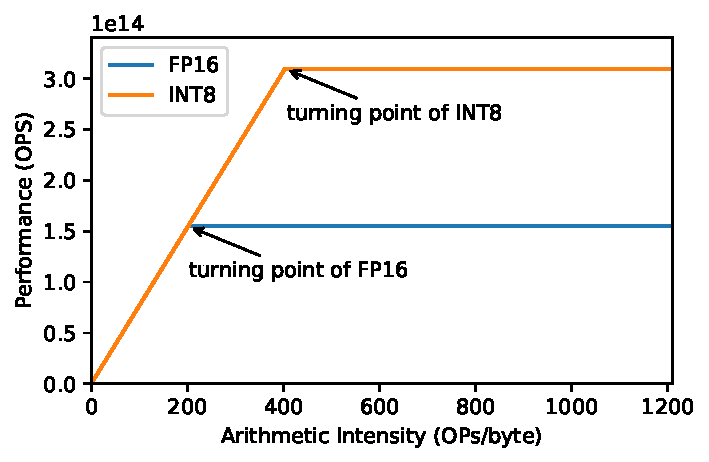
\includegraphics[width=0.95\linewidth]{ims/quantization_roofline_model.pdf}
    % \vspace{-0.6in}
    \caption{Demonstration of the Roofline model of Nvidia A6000 GPU for different computation data types.}
    \label{fig:quantization_roofline_model}
\end{figure}

\begin{figure}[t]
    \centering
    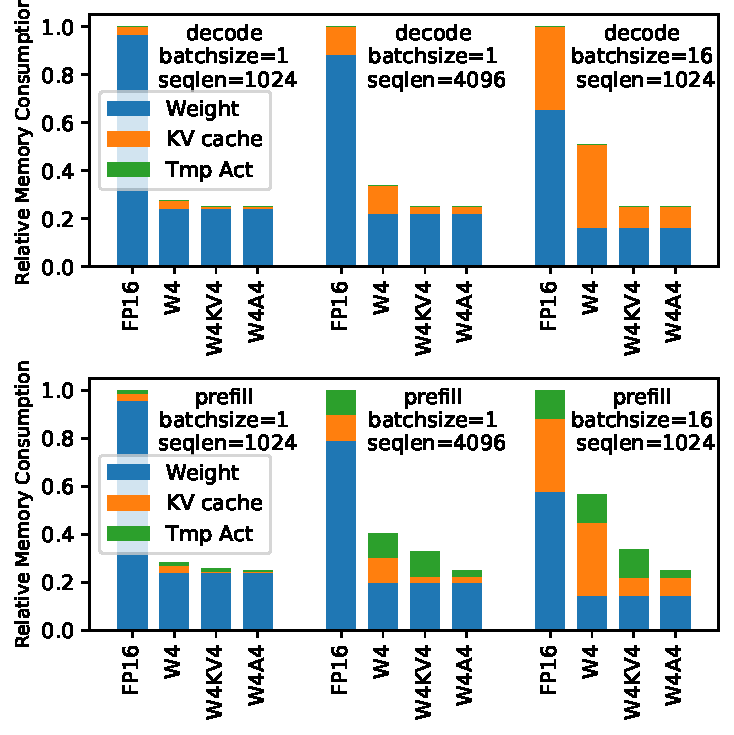
\includegraphics[width=0.95\linewidth]{ims/quantization_memory_consumption.pdf}
    % \vspace{-0.6in}
    \caption{Relative memory consumption for different quantization settings for Llama-2-13b. Tmp Act means temporary activations.}
    \label{fig:quantization_memory_consumption}
\end{figure}

\textbf{Computation}: 
The latest computing devices, such as NVIDIA GPUs, generally support FP32, FP16, and INT8 data types for computation. Hardware devices generally perform better when processing data with smaller bit widths. NVIDIA's A6000 GPU, for example, is capable of performing twice as fast as FP16 with 155 TOP/s and 310 TOP/s, respectively.
In the Roofline model, when enabling quantization for faster computation, the roofline height increases, indicating improved performance for compute-bound layers. 
As shown in Figure~\ref{fig:quantization_roofline_model}, the max performance improved when using INT8 computation.
However, to utilize the computational power of INT8, all input operands must be in INT8 format. Consequently, if only the weights are quantized to INT8 while the activations remain in FP16 format, the INT8 computational power cannot be utilized. Instead, the INT8 weights would need to be converted to FP16 for multiplication with FP16 activations.
Furthermore, when tensors are quantized to a bitwidth that is not supported by the hardware, they need to be converted to higher bit widths for computation. For example, the NVIDIA H100 GPU does not support INT4 computation. Consequently, if the weight or activation is quantized to INT4, it would require conversion to a higher bit width, such as INT8 or FP16, for computation.

\textbf{Memory Consumption}: The memory consumption reduction resulting from quantizing different tensors varies, as shown in Figure~\ref{fig:quantization_memory_consumption}~\footnote{In our notation, W4 represents the quantization of weights to 4 bits while keeping activations in FP16 format. W4A4 indicates both weights and activations quantized to 4 bits. In the case of W4KV4, weights and the KV cache are quantized, while temporary activations remain in FP16 format.}. Notably, the memory usage of temporary activations is relatively low, especially during the decode stage. This can be attributed to their short lifespan, allowing their memory to be released once their purpose is fulfilled.
On the other hand, the memory allocated for the KV cache behaves differently. It cannot be freed until the entire process of generating a complete answer is finished, which entails multiple inference passes through the network. Additionally, the memory consumption of the KV cache increases as the batch sizes grow larger and the input sequences become longer. This is because the model needs to store a greater number of key-value (KV) pairs to facilitate its operations.

\textbf{Memory Access}: Quantizing tensors in LLM can significantly reduce memory access, resulting in fewer data bytes to be moved for the same amount of computation. This increase in arithmetic intensity contributes to the Roofline model, leading to three scenarios:
(1) After quantization, the arithmetic intensity remains within the memory-bound range. With the improvement in arithmetic intensity, the average data access per computation is reduced, alleviating the pressure on data memory access. Consequently, the theoretical performance is enhanced. This can greatly boost the performance during the memory-bound decode stage.
(2) The arithmetic intensity transitions from being memory-bound to compute-bound. This shift also reduces the pressure on data memory access, resulting in improved theoretical performance.
(3) Both before and after quantization, the arithmetic intensity remains within the compute-bound range. In this case, there is no performance improvement. For example, this scenario can occur during the compute-bound prefill stage or when the batch size is large in the decode stage.

As depicted in Figure~\ref{fig:quantization_memory_access_batch}, when the batch size is small, the layers in the network are memory-bound both before and after quantization. Therefore, quantization can enhance performance and reduce the network's inference time. However, when the batch size is large, compressing the network's weights from 4 bits to 2 bits or 1 bit does not lead to a decrease in the inference time. This is because, at this point, the network is already compute-bound, and quantizing the weights becomes ineffective.
Similar to the previous scenario, the behavior of the system can exhibit saturation effects in prefill stage. As shown in Figure~\ref{fig:quantization_memory_access_seq_len}, when the sequence length is relatively small, the prefill stage is memory-bound. In this case, applying quantization can enhance the performance by reducing the memory access requirements of the network.
However, as the sequence length increases, the prefill stage becomes more compute-bound. Consequently, quantizing the weights may not yield significant improvements in performance when the network is already compute-bound during the prefill stage with large sequence lengths.

% 对于prefill阶段，当sequence length发生变化时，也会出现这种“饱和”的现象。如图所示，当sequence length较小时，prefill阶段是compute-bound，量化可以提升performance；但当sequence length较大时
% As shown in Figure~\ref{quantization_memory_access_batch}, 在batch size较小的情况下，网络中的layers在量化前后都是memory-bound的，因此对量化可以增加performance，从而减少网络的inference time。 然而在batch size较大的情况下，将网络中的权重从4bit压缩到2bit或者1bit没有the inference time的减少，这就是因为这个时候已经是compute-bound，对权重进行量化已经没有用了。

\begin{figure}[t]
    \centering
    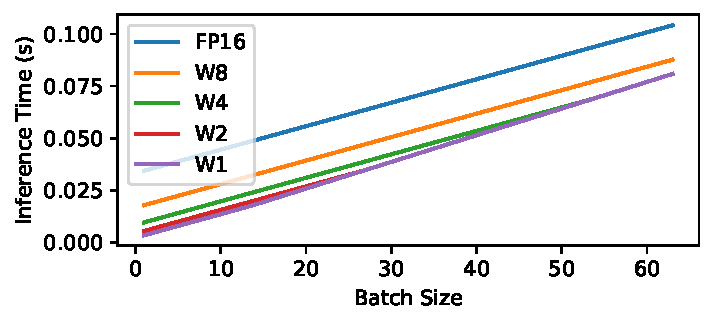
\includegraphics[width=0.95\linewidth]{ims/quantization_memory_access_batch.pdf}
    % \vspace{-0.6in}
    \caption{Inference time of decoding stage for different quantization settings on Llama-2-13b. (Sequence length=1024)}
    \label{fig:quantization_memory_access_batch}
\end{figure}

\begin{figure}[t]
    \centering
    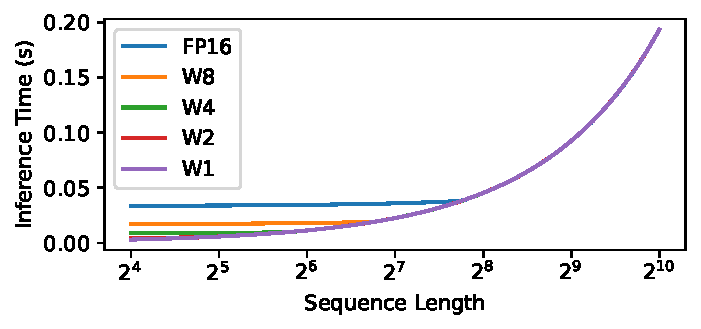
\includegraphics[width=0.95\linewidth]{ims/quantization_memory_access_seq_len.pdf}
    % \vspace{-0.6in}
    \caption{Inference time of prefill stage for different quantization settings on Llama-2-13b. (Batch size=1)}
    \label{fig:quantization_memory_access_seq_len}
\end{figure}

% 量化各个tensor可以大幅度减少memory access，相同计算量所需搬运的数据bytes少了，从而增加Roofline model中的arithmetic intensity。量化后layer的arithmetic intesity的虚线将会向右移动，这会导致三种情况：(1) 量化后arithmetic intensity都在memory bound区间，由于arithmetic intensity提升了，平均一次计算所需的数据access更小了，缓解了数据的访存的压力，因此理论performance也得到了提升。这能大幅度提升在memory-bound的decode阶段性能。 (2) arithmetic intensity从memory-bound变成了compute-bound，这也环节了数据访存压力，提升理论performance。(3) 量化前后arithmetic intensity都在compute-bound，这种情况下没有性能提升。例如compute-bound的prefill阶段或者batchsize很大的decode阶段。

% Based on above observations, we believe that exclusively quantizing the weights and KV cache is a favorable choice. However, not quantizing temporary activations has two drawbacks: increased memory usage and the inability to utilize faster computation units, such as Nvidia's INT8 acceleration units. Nevertheless, these drawbacks do not significantly impact network inference. Firstly, as discussed earlier, temporary activations occupy minimal memory. Secondly, the unavailability of faster computation units does not greatly affect the inference speed. Figure~\ref{im_time} shows that the time cost of weight-KV cache quantization is nearly the same as weight-activation quantization. This is because the inference of LLMs is primarily constrained by memory access. Therefore, exclusive quantization of weights and KV cache is a beneficial trade-off between retaining model accuracy and achieving memory savings when compared to quantizing both weights and activations. 

\subsubsection{Quantization for Compressing Pre-trained LLMs}
In Quantization-Aware Training (QAT)~\citep{courbariaux2015binaryconnect,choi2018pact,dong2019hawq}, the quantization process is seamlessly integrated into the training of Large Language Models (LLMs), enabling them to adapt to low-precision representations and thus mitigating precision loss. LLM-QAT~\citep{liu2023llm} innovatively addresses the challenge of training data acquisition for LLMs through data-free distillation, which leverages outputs from a pre-trained model to obviate the need for extensive data collection. Furthermore, LLM-QAT expands quantization beyond weights and activations to include key value (KV) caches, enhancing throughput and supporting longer sequence dependencies. Its successful distillation of large Llama models to 4-bit quantized weights and KV caches underscores the potential for accurately quantized 4-bit LLMs.

To attain lower-bit quantization, such as below 2-bit, \cite{kim2023token} introduce Token-Scaled Logit Distillation (TSLD) for ternary QAT in LLMs. This method employs an adaptive knowledge distillation technique that modifies Logit Knowledge Distillation based on token confidence, providing tailored guidance during LLM QAT. Furthermore, \cite{shang2024pb} focus on salient weights with their concept of partially binarized matrices in PB-LLM. By preserving these crucial weights in higher bits, PB-LLM effectively maintains the reasoning capacity of heavily quantized LLMs. Additionally, PB-LLM explores minimizing quantization error by determining the optimal scaling factors for binarized LLMs, a vital step in preserving the effectiveness of models under aggressive quantization.

\begin{figure*}[t]
    \centering
    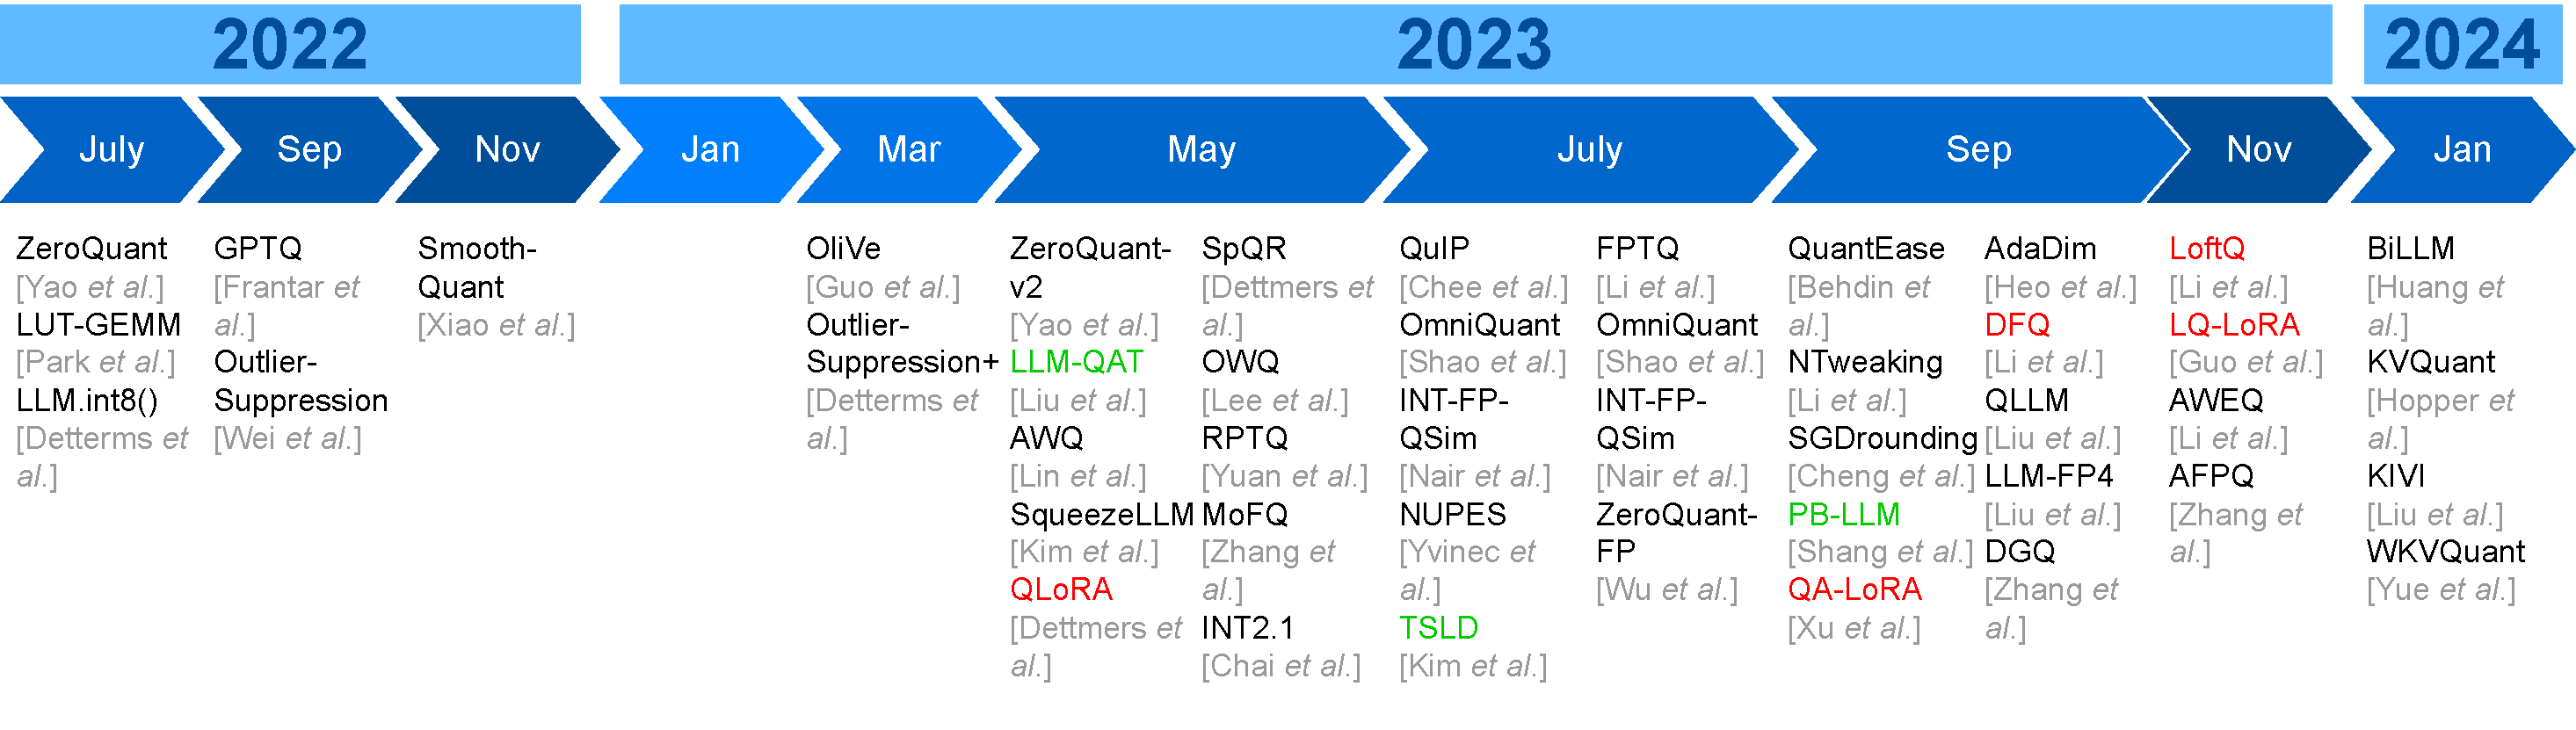
\includegraphics[width=0.99\linewidth]{ims/quantization-timeline-2024feb.pdf}
    \vspace{-0.1in}
    \caption{Timeline of Quantization for LLM methods from 2022 to 2024. The \textcolor{red}{red}-highlighted methods represent they belonging to Quantization for Parameter Efficient Fine-Tuning (Q-PEFT), the \textcolor{green}{green}-highlighted methods represent they belonging to QAT-related methods, and others are PTQ-based methods.}
    \label{fig:ptq-timeline}
\end{figure*}
 
\noindent\textbf{Post-Training Quantization (PTQ)}

Post-Training Quantization (PTQ) represents a crucial technique in optimizing Large Language Models (LLMs), entailing the quantization of model parameters post the LLM's training phase. The primary goal of PTQ is to reduce both the storage requirements and computational complexity of the LLM, without necessitating alterations to the model's architecture or embarking on a retraining process. This approach stands out for its simplicity and efficiency, particularly in achieving significant model compression. In the context of LLMs, which typically contain billions of parameters, Quantization-Aware Training (QAT) often becomes impractical due to excessive training costs. Hence, PTQ emerges as a more viable solution for these large-scale models. However, it's crucial to acknowledge that PTQ can lead to a certain degree of precision loss as a consequence of the quantization process. Despite this, PTQ serves as an effective method to enhance the efficiency of LLMs, offering a straightforward solution that avoids major modifications or extensive additional training.

In PTQ, various approaches focus on \textbf{weight-only quantization} to enhance efficiency. For instance, LUT-GEMM~\citep{park2023lut} optimizes matrix multiplications in LLMs using weight-only quantization and the BCQ format, thereby reducing latency and improving computational efficiency. 
 LLM.int8()~\citep{dettmers2022llm} employs 8-bit quantization, which halves GPU memory usage during inference and maintains precision through vector-wise quantization and mixed-precision decomposition. This method enables efficient inference in models up to 175 billion parameters. 
ZeroQuant~\citep{yao2022zeroquant} combines a hardware-friendly quantization scheme with layer-by-layer knowledge distillation, optimizing both weights and activations to INT8 with minimal accuracy loss. 
Addressing higher compression targets, GPTQ~\citep{frantar2022gptq} introduces a layer-wise quantization technique based on approximate second-order information, achieving a reduction to 3-4 bits per weight with minimal accuracy loss. Additionally, the study by \cite{dettmers2023case} explores the balance between model size and bit precision, particularly for zero-shot performance, finding that 4-bit precision generally offers the optimal balance.
Innovations like AWQ~\citep{lin2023awq, kim2023squeezellm} highlight that protecting a small percentage of salient weights can significantly reduce quantization error. AWQ uses an activation-aware approach, focusing on weight channels with larger activation magnitudes, and incorporates per-channel scaling for optimal quantization. OWQ~\citep{lee2023owq} analyzes how activation outliers amplify quantization error, introducing a mixed-precision scheme to assign higher precision to weights affected by these outliers. SpQR~\citep{dettmers2023spqr} takes a unique approach by isolating outlier weights for storage in higher precision, while compressing the remainder to 3-4 bits. This technique allows for more efficient compression while maintaining near-lossless performance.
QuantEase~\citep{behdin2023quantease} suggests using a coordinate descent approach to optimize all of the weights in network, improving the efficiency of quantization.


To achieve even lower-bit quantization (e.g., below 2-bit), QuIP~\citep{chee2023quip} introduces an innovative approach that accounts for the even distribution of weight magnitudes and the significance of accurately rounding directions unaligned with coordinate axes. QuIP comprises an adaptive rounding procedure that minimizes a quadratic proxy objective, essential for optimizing the quantization process. Additionally, it employs efficient pre- and post-processing techniques that ensure weight and Hessian incoherence through multiplication by random orthogonal matrices, crucial for maintaining quantization effectiveness.
Further advancing PTQ methods, \cite{li2023norm} are inspired by the observation that aligning the quantized activation distribution with its floating-point counterpart can restore accuracy in LLMs. Their proposed 'Norm Tweaking' strategy involves a meticulous calibration data generation process and a channel-wise distance constraint. This approach updates the weights of normalization layers, leading to enhanced generalization capabilities.
\citep{shang2024pb}~propose partial-binarized LLM (PB-LLM) by introducing binarization~\citep{hubara2016binarized}~into LLM quantization to push weight quantization under 2 bits. Following PB-LLM, BiLLM~\citep{huang2024billm} pushes weight quantization to almost 1 bit.

% Each of these PTQ methods demonstrates innovative strategies to tackle the challenges of quantizing LLMs while preserving accuracy and efficiency. From QuIP's adaptive rounding procedure to Norm Tweaking's focus on activation distribution alignment, these approaches showcase the diverse and sophisticated techniques being developed in the field of LLM optimization. These advancements reflect a deep understanding of the complexities inherent in LLM quantization, highlighting the ongoing efforts to enhance model performance and efficiency in this rapidly evolving domain.

Apart from efforts that focus solely on weight quantization in LLMs, numerous PTQ approaches focus on \textbf{weights and activations quantization}. SmoothQuant~\citep{xiao2023smoothquant} addresses the challenge of quantizing activations, which can be complex due to the presence of outliers. It introduces a per-channel scaling transformation that effectively smooths out activation magnitudes, rendering the model more receptive to quantization.
Recognizing the intricacies of quantizing activations in LLMs, RPTQ~\citep{yuan2023rptq} highlights the uneven ranges across channels and the prevalence of outliers. RPTQ's innovative approach involves clustering channels for quantization, thereby reducing discrepancies in channel ranges. This method smartly integrates channel reordering into layer normalization and linear layer weights to minimize overhead.
OliVe~\citep{guo2023olive} adopts an outlier-victim pair (OVP) quantization strategy, focusing on local handling of outliers with low hardware overhead and significant performance benefits. This approach stems from the understanding that outliers are crucial, while adjacent normal values are less so. Building on this, Outlier Suppression+ extends the concept by addressing asymmetrically distributed harmful outliers in specific channels. It introduces channel-wise shifting and scaling operations to balance the outlier distribution and reduce the impact of problematic channels, considering both the nature of the outliers and the subsequent quantization errors.
ZeroQuant-FP~\citep{wu2023zeroquant} delves into floating-point (FP) quantization, specifically exploring FP8 and FP4 formats. This study finds that FP8 activation quantization in LLMs outperforms the traditional INT8 format, while FP4 weight quantization shows comparable efficacy to INT4. ZeroQuant-FP addresses the divergence between weights and activations by standardizing all scaling factors as powers of 2 and restricting them within a single compute group, ensuring consistency and efficiency in the quantization process.
\cite{li2023fptq} propose FPTQ, in which they employ a layerwise strategy to cope with different levels of quantization difficulty. Particularly, they devises an offline logarithmic activation equalization to render a quantization-friendly distribution for previously intractable layers.

\begin{figure}[t]
    \centering
    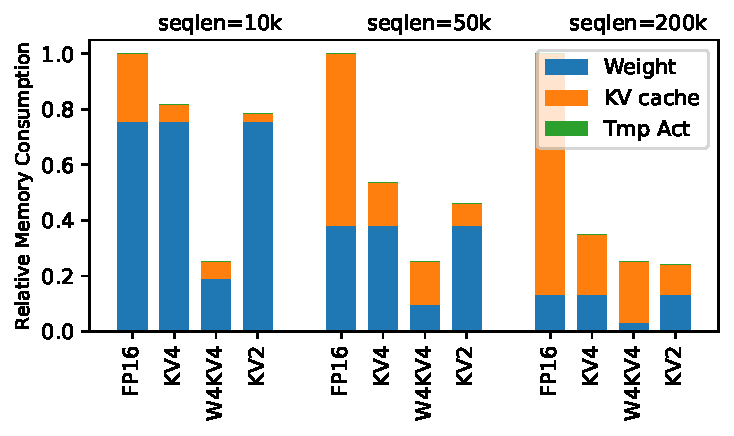
\includegraphics[width=0.95\linewidth]{ims/quantization_memory_consumption_long_seq.pdf}
    % \vspace{-0.6in}
    \caption{Memory Consumption of decode stage for different quantization settings on Llama-2-13b. (Batch size=1).}
    \label{fig:quantization_memory_consumption_long_seq}
\end{figure}

Since the end of 2023, the length of tokens has been significantly increasing, causing the KV cache to consume more memory. 
For instance, Google Gemini 1.5~\citep{gemini2024} can handle up to 1 million tokens in production, and LLMs processing books, large images or videos will require tens of thousands of tokens. As a result, the optimization of \textbf{KV Cache Quantization} has become increasingly important. 
Several recent papers in 2024 have focused on improving KV cache quantization. 
For example, \cite{hooper2024kvquant} propose a solution for achieving 10 million context length LLM inference with KV Cache Quantization.
KIVI~\citep{liu2024kivi} pushes the quantization of KV cache to 2-bit.
\cite{yue2024wkvquant} proposes WKVQuant as to jointly optimize the quantization of both the weights and the KV cache in LLMs, making W4KV4 have the same performance as W4.
As shown in Figure~\ref{fig:quantization_memory_consumption_long_seq}, we use LLM-Viewer to analyze the memory reduction of KV cache quantization.
We can observe that when the sequence length is larger than 50k, the KV cache takes most of the memory and its quantization can significantly decrease the memory consumption.

% Recently, the sequence length is becoming larger, resulting in that the KV cache takes much more memory. For example, Google Gemini 1.5~\cite{gemini2024} run up to 1 million tokens in production, and LLM that process the video can takes millions of tokens. 
% Therefore, \textbf{KV Cache Quantization} is becoming more and more important. 
% There are recent paper are optimized for better KV cache quantization.
% \citep{yue2024wkvquant} identifies the huge cost from key/value (KV) cache, and propose WKVQuant for quantizing weights and the KV cache of LLMs.


\subsubsection{Quantization for Parameter Efficient Fine-Tuning (Q-PEFT)}

\textbf{Parameter Efficient Fine-Tuning (PEFT)} is an important topic for LLMs. One of the most popular approaches is low-rank adaptation (LoRA)~\citep{hu2021lora,valipour2022dylora}, where the key insight is to decompose the adapter weights into the multiplication of two low-rank (and thus parameter-efficient) matrices. 
LoRA has claimed comparable performance to full fine-tuning while using much fewer learnable parameters. 
Please refer to the review paper~\citep{hu2023llm} for more details about this adaptor. 

In addition to the well-defined quantization paradigms, a novel paradigm in LLM efficiency is emerging: Quantization for Parameter-Efficient Fine-Tuning (Q-PEFT).
This approach integrates quantization into the fine-tuning process of LLMs, offering a unique and efficient method, particularly relevant in the era of large models. 
Pioneering works in this paradigm, such as PEQA~\citep{kim2023memory}, DFT~\citep{li2023qft}, and QLORA~\citep{dettmers2023qlora} demonstrate the feasibility and effectiveness of this approach. 
PEQA employs a dual-stage process where the first stage involves quantizing the parameter matrix of each fully connected layer into a matrix of low-bit integers coupled with a scalar vector. The second stage focuses on fine-tuning the scalar vector for specific downstream tasks, allowing for more efficient task-specific adjustments. 
DFT adopts the efficient Lion optimizer, which only keeps track of the momentum and has consistent update magnitudes for each parameter, an inherent advantage for robust quantization; and (ii) we quantize all model states and store them as integer values, and present a gradient flow and parameter update scheme for the quantized weights. 
On the other hand, QLORA introduces novel concepts such as a new data type, double quantization, and paged optimizers. These innovations aim to conserve memory efficiently while maintaining LLM fine-tuning performance. Notably, QLORA facilitates large model fine-tuning on a single GPU, achieving state-of-the-art results on the Vicuna benchmark, a testament to its effectiveness in balancing memory efficiency and model performance.


However, a limitation of QLoRA is its restriction to at most 4-bit quantization during fine-tuning; lower-bit quantization, such as 2-bit, can significantly deteriorate the performance. Addressing this challenge, several studies have ventured into the realm of Q-PEFT to enable lower-bit quantization. LQ-LoRA~\citep{guo2023lq} introduces an iterative algorithm that decomposes each pretrained matrix into a high-precision, low-rank component and a memory-efficient quantized component. During fine-tuning, only the low-rank component is updated, keeping the quantized component fixed. This method presents an integer linear programming approach for the quantization component, allowing dynamic configuration of quantization parameters like bit-width and block size within a given memory budget. Another notable approach, Loft-Q~\citep{li2023loftq}, simultaneously quantizes an LLM and establishes a suitable low-rank initialization for LoRA fine-tuning. This strategy effectively bridges the gap between the quantized and full-precision models, significantly enhancing generalization in downstream tasks. 
QA-LoRA~\citep{xu2023qa} leverages the benefits of quantizing the LLM’s weights into low-bit integers, facilitating an efficient fine-tuning stage. Additionally, it produces a lightweight, fine-tuned model, circumventing the accuracy loss often associated with PTQ.



\subsubsection{Discussion on LLM Quantiztaion}
Figure~\ref{fig:ptq-timeline} presents a timeline of LLM quantization techniques, highlighting the evolution from Post-Training Quantization (PTQ) as the initial mainstream approach to the rising prominence of Quantization-Aware Training (QAT) and Quantization for Parameter-Efficient Fine-Tuning (Q-PEFT). This shift underscores the community's adaptation in response to the performance bottlenecks encountered with PTQ, marking QAT and Q-PEFT as the burgeoning areas of focus in the quest for efficient LLM inference.
% \subsubsection{Discussion on LLM Quantiztaion}
% Figure~\ref{fig:ptq-timelin} illustrates the timeline of LLM quantization. 
% We depict the development of DFKD and SFDA on the upper and lower stream, respectively.



\subsection{Pruning}
Pruning~\citep{lecun1989optimal,liang2021pruning}, which concentrates on identifying and eliminating model parameters that are deemed unnecessary or redundant, is another popular technique for compressing LLMs.
In the context of LLMs, the parameters often account for a considerable portion of the model size and computational demand. By carefully pruning these parameters, it's possible to streamline the model, making it more efficient without significantly compromising its performance. 
Pruning methods can be broadly classified into two categories: unstructured pruning and structured pruning, and we describe the research progress of each category in turn below.

\subsubsection{Unstructured pruning} 
Unstructured pruning selectively eliminates individual weights or neurons from a model, leading to a sparser, yet more irregularly structured network. This form of pruning excels in ensuring model accuracy, however, the resultant irregularity in the weight distribution necessitates specialized handling or software optimizations.
SparseGPT~\citep{frantar2023sparsegpt} is a groundbreaking one-shot pruning method tailored for LLMs. It tackles the pruning challenge by reconceptualizing it into a series of extensive sparse regression problems, efficiently solved by a newly developed solver. Notably, SparseGPT can efficiently process a model with 175 billion parameters in just a few hours on a single GPU, and it can induce significant sparsity (50-60\%) in LLMs without significantly sacrificing accuracy or necessitating fine-tuning. 
To tackle the challenge of reconstruction cost in SparseGPT, \cite{sun2023simple} propose Wanda, which assesses the significance of each weight by evaluating its magnitude and the norm of the corresponding input, significantly increasing the computational efficiency.
Further, \cite{yin2023outlier} design a set of non-uniform hierarchical sparsity ratios to pay more attention to the layers with higher outlier occurrences, thus boosting the pruning performance.
Moreover, Considering the hardware support for unstructured pruning, Flash-LLM~\citep{xia2023flash} proposes an unstructured sparse matrix multiplication method, which is characterized by sparse loading and dense computation, to implement the GPU Tensor Core's sophisticated support for unstructured sparsity.


\subsubsection{Structured pruning} 
Structured pruning removes entire neurons or layers, resulting in a cleaner, more regular structure. The pruned model is generally more compatible with conventional hardware, however, the simplicity and regularity come at a cost: this form of pruning can have a more pronounced impact on the model's performance, as it involves removing larger, potentially more critical components.
LLM-Pruner~\citep{ma2023llm} represents a pioneering approach in structural pruning for LLMs. It employs a one-shot pruning technique, which relies on first-order and estimated Hessian data and necessitates subsequent fine-tuning using LoRA to restore the weights. This work is advantageous as it significantly reduces both computational demands and memory requirements, while preserving the fundamental structure of LLMs. 
Sheared Llama~\citep{xia2023sheared} proposes another noteworthy solution by combining targeted structured pruning with a dynamic batch loading algorithm. First, it meticulously prunes a source model into a desired target architecture, meticulously chosen by analyzing the configurations of the pre-trained model. Then, it enhances training efficiency through the dynamic batch loading algorithm, which adjusts the proportion of training data from various domains.
Compresso~\citep{guo2023compresso} establishes a collaborative learning framework, where the LLM and a resource-efficient pruning algorithm work in tandem, with the ability to prune Llama-7B to 5.4B while preserving the original performance.


\subsection{Knowledge Distillation}
Knowledge distillation~\citep{hinton2015distilling,gou2021knowledge} is a technique that facilitates the transfer of capabilities from a larger model (referred to as the ``teacher'') to a smaller model (referred to as the ``student''), allowing the smaller model to perform tasks with similar proficiency as the larger model but with reduced computational resources~\citep{gou2021knowledge,shang2021lipschitz}. 
For LLM compression, there are two main categories of knowledge distillation: white-box and black-box distillation. Within these categories, researchers have developed a range of distillation methods tailored for LLMs, which are described in detail below. 
Moreover, a more detailed and specific survey regarding knowledge distillation of LLMs has also been carried out~\citep{xu2024kdsurvey}. 

\subsubsection{White-Box Knowledge Distillation}
In white-box distillation, the architecture and weights of the teacher model are fully accessible. This transparency allows the student model to learn not just the output of the teacher model but also its internal representations and decision-making processes.
MiniLLM~\citep{gu2023knowledge} critiques the limitations of standard knowledge distillation objectives and suggests that reverse Kullback-Leibler divergence is more effective for capturing the complexity of generative tasks, which can enhance the student model's response quality and reliability. MiniLLM also introduces single-step regularization, teacher-mixed sampling, and length normalization to address challenges in training, thus demonstrating great performance potential for distilling LLMs on the standard benchmarks.
In contrast to MiniLLM, GKD~\citep{agarwal2023gkd} presents a more straightforward and stable method. It aligns more with supervised training by avoiding backpropagation through the student model’s sampling. Instead of using predetermined output sequences, GKD trains the student model on its own created sequences, utilizing the teacher's probabilities as guidance, which leads to notable improvements in the student's performance.
Homotopic distillation~\citep{liang2023homodistil} aims to facilitate the alignment of the student model's predictions with those of the teacher model across extensive open-domain data. It involves starting the student model with the teacher model's configuration and progressively reducing the student model's neurons to reach a specified model complexity.
Furthermore, ~\cite{liang2023less} present a layerwise distillation approach that involves creating unique task-aware filters for each layer of teacher and student models. These filters, essentially neural networks equipped with task-specific heads, are designed to distill and capture the predictive knowledge from the hidden layers of the respective models.
AD-KD~\citep{wu2023ad} analyzes the teacher model's token-level rationale using integrated gradients and transfers attributional knowledge to the student model, which enables the student model to imitate the teacher's underlying reasoning, not just its behaviors.



\subsubsection{Black-Box Knowledge Distillation}
Contrary to white-box distillation, black-box distillation does not require access to the internal information of the teacher model. Instead, it focuses on replicating the output behavior of the teacher model. The student model learns solely from the input-output pairings produced by the teacher, without any insight into its internal operations.
Multitask-ICT~\citep{huang2022context} introduces in-context learning distillation, which merges the objectives of in-context learning with those of language modeling, intending to distill into smaller models both the capability to comprehend in-context examples and the knowledge required for specific tasks.
LaMini-LM~\citep{wu2023lamini} creates a set of 2.58 million instructions and employs GPT-3.5 Turbo to produce responses to these instructions. Subsequently, it uses these instructions as a basis to fine-tune a range of student models.
Similarly proceeding from creating examples, ~\cite{sahu2023promptmix} proposes PromptMix, which involves a two-step method based on prompting to create labeled examples for text classification. In PromptMix, the borderline examples can enhance the knowledge transfer from teacher models like GPT-3.5 to student models.
In contrast to the traditional unidirectional knowledge distillation, Lion~\citep{jiang2023lion} introduces an adversarial distillation framework, which encourages the teacher model to identify "hard" instructions and subsequently generate new "hard" instructions for the student model, resulting in a dynamic three-step adversarial cycle.
% ~\citep{chen2023disco}

Black-box distillation is also identified as a promising tool to transfer the power of chain-of-thought (CoT) prompting from larger models to smaller ones.
~\cite{fu2023specializing} observe a trade-off in language models between their diverse capabilities, and focus on moving the teacher model's capability from general abilities towards enhancing the student model's proficiency in the targeted mathematical CoT.
SCOTT~\citep{wang2023scott} uses contrastive decoding for better rationale supervision and a counterfactual reasoning objective for faithful distillation, resulting in more faithful CoT rationales.
Distilling step-by-step~\citep{hsieh2023distilling} introduces a novel training method for smaller models, surpassing LLMs with less data. It uses LLM rationales as extra training material in a multi-task framework, cutting down data needs versus standard fine-tuning and distillation.
Similarly, ~\cite{li2023symbolic} propose symbolic CoT distillation, where they obtain CoT rationales for unlabeled dataset instances from the teacher model and then train the student model to forecast both the rationale and the label based on these instances.
To promote complex, multi-step reasoning within a dialogue context, i.e., dialogue CoT reasoning, ~\cite{chae2023dialogue} utilize LLMs as inconsistent teachers and strategically distill valuable and logical rationales through alignment filters.



\subsection{Factorization}
% In the content of LLM compression via decomposition, the most related work is TensorGPT~\cite{xu2023tensorgpt}, in which the embedding layer of LLMs is compressed through Tensor-Train Decomposition (TTD)~\cite{oseledets2011tensor} in order to store large embeddings in a low-rank tensor format, with much fewer parameters. However, there are several differences between those two methods: 
% (1) Unlike TensorGPT which focuses solely on the token embedding matrix, ASVD aims to compress the entire weight spectrum of LLMs. This holistic approach addresses a more critical aspect of LLM compression, as highlighted in recent studies; 
% (2) From the perspective of low-rank decomposition categorization, our method can realize the low-rank decomposition in a rank-adaptive manner, contrasting with the fixed or predetermined ranks used in TensorGPT. 
The use of low-rank matrix decomposition~\citep{kishore2017literature} as a technique for compressing Deep Neural Networks (DNNs) represents a straightforward yet effective approach, garnering considerable attention within both scientific computing and machine learning domains. In recent years, the challenge of efficiently compressing and accelerating large-scale neural networks via low-rank methods has become a focal point of research. This has led to significant advancements in developing and refining low-rank factorization strategies tailored for DNNs~\citep{schotthofer2022low}. 

Activation-aware Singular Value Decomposition (ASVD)~\citep{yuan2023asvd} is the first work using factorization techniques to compress LLM. 
ASVD effectively manages activation outliers by adjusting the weight matrix based on the activation distribution, improving decomposition accuracy and efficiency. ASVD also addresses the varying sensitivity of different LLM layers to decomposition, with an iterative calibration process for optimal layer-specific decomposition.
Concurrently, LAyer-SElective Rank reduction (LASER)~\citep{sharma2023truth} demonstrates the surprising result that it is often possible to significantly improve the performance of LLMs by selectively removing higher-order components1 of their weight matrices. 
Apart from targeting the LLMs' weights, TensorGPT~\citep{xu2023tensorgpt}, in which the embedding layer of LLMs is compressed through Tensor-Train Decomposition (TTD)~\citep{oseledets2011tensor} in order to store large embeddings in a low-rank tensor format, with much fewer parameters. 